\begin{frame}
\frametitle{Real Word Error Correction} 
\centering
\begin{figure}
    \centering
    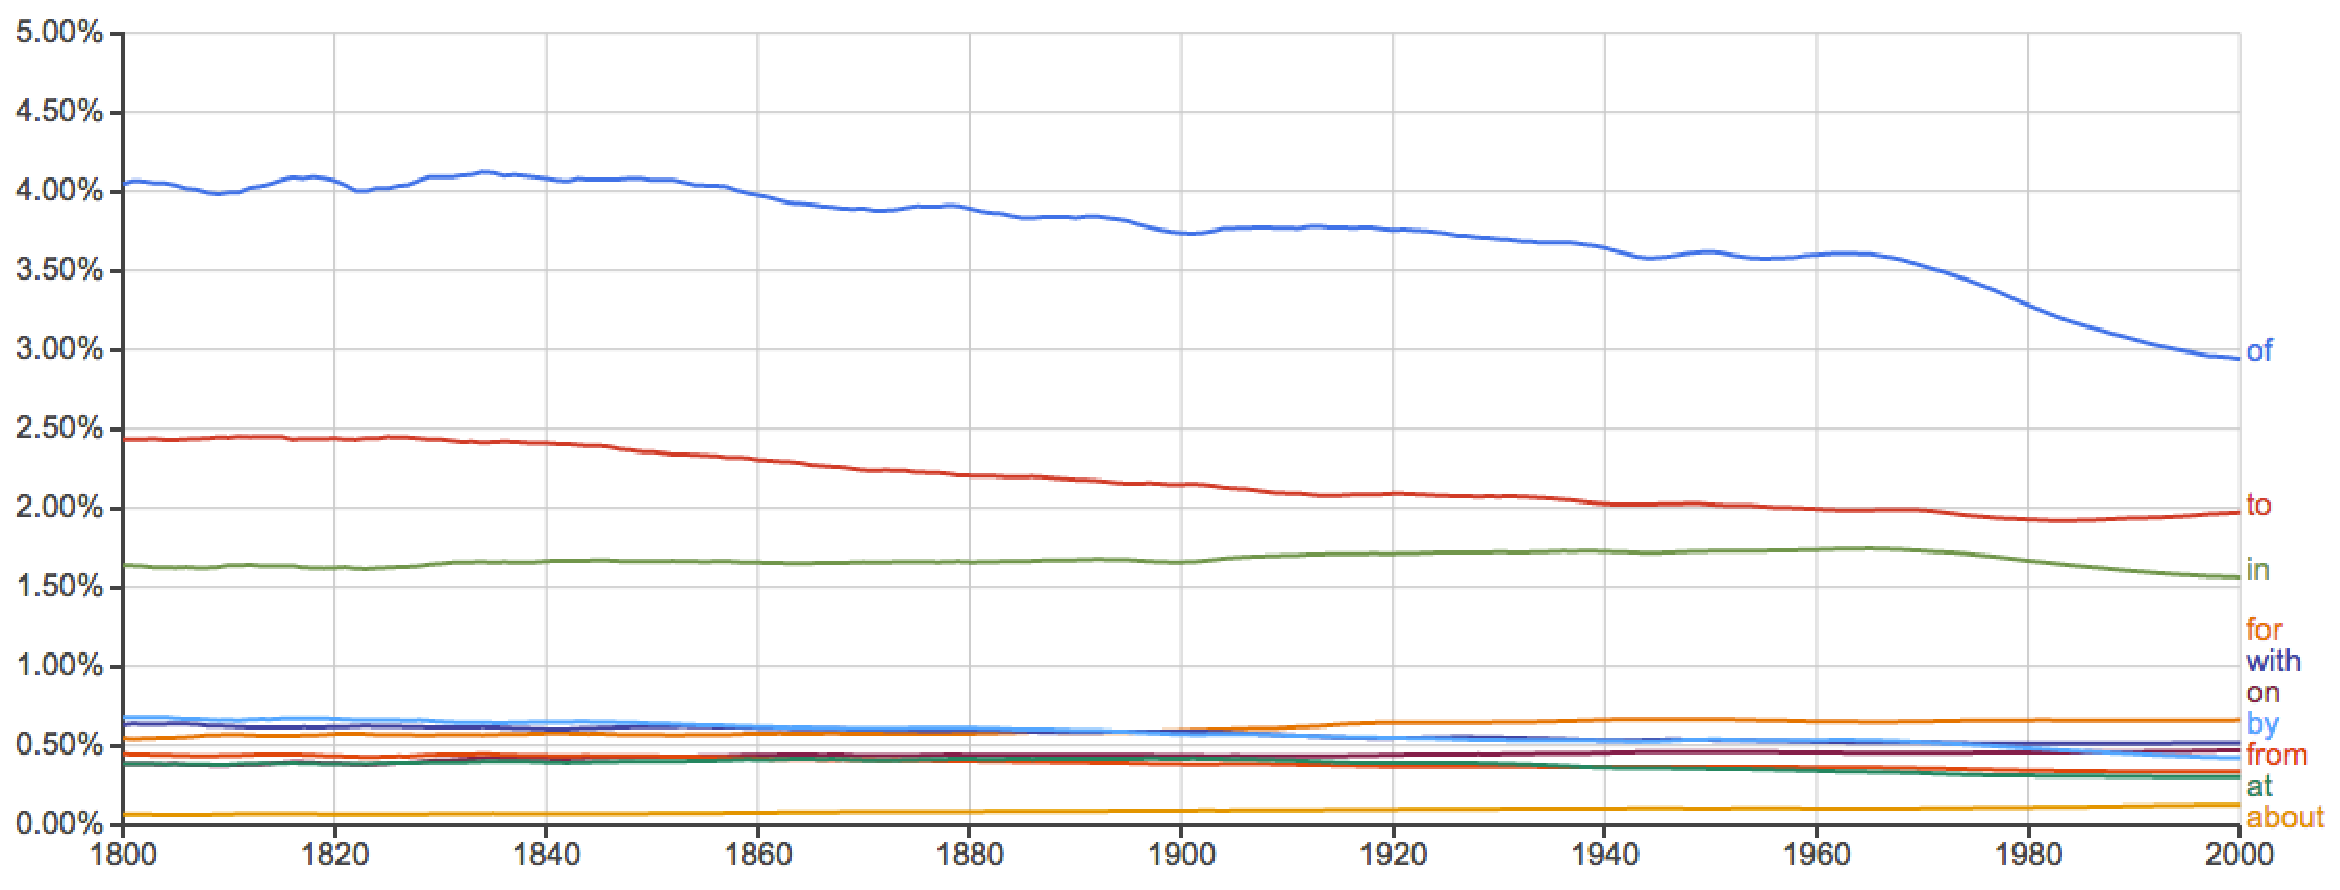
\includegraphics[width=\textwidth]{figures/chapter06/preposition-frequencies}
    \caption{Relative frequencies of 10 prepositions.  Our confusion set consists of all but the least frequent, ``about''.}
\end{figure}
\end{frame}

\begin{frame}
\frametitle{Contrasting Cases}
\begin{table}
\begin{tabular}{cc}
\textbf{Sentence} & \textbf{Target} \\
\hline
This is justified \textbf{on} policy grounds. & \textbf{on} \\
This is justified \textbf{for} policy grounds. & \textbf{on} \\
\hline
\end{tabular}
\caption{A ConvNet trained to predict the preposition that exists in the sentence learns to copy the preposition and ignore its context.  Training with contrasting cases prevents the trivial solution and forces the model to focus on the context of the preposition.} 
\end{table}
\end{frame}

\begin{frame}
\frametitle{Real Word Error Correction Data}
\begin{itemize}
    \item Sentences from English Wikipedia 
    \item {\textasciitilde}75m training ({\textasciitilde}37.5m contrasting cases)
    \item 1m validation (500k contrasting cases) 
    \item 1m test (500k contrasting cases) 
\end{itemize}
\end{frame}

\begin{frame}
\begin{table}
\centering
\begin{tabular}{lrr}
\hline
Inputs & Filter width & Acc. \\
\hline
\textbf{Window9} & 7 &  .801 \\
\textbf{Window9}$\oplus$\textbf{Sentence} & 9 &  .800 \\
\textbf{Window5}$\oplus$\textbf{Sentence} & 5 &  .800 \\
\textbf{Window7}$\oplus$\textbf{Sentence} & 7 &  .798  \\
\textbf{Window7} & 5 &  .794 \\
\textbf{Window5} & 3 &  .765 \\
\textbf{Sentence} & 5 &  .732 \\
\hline
\end{tabular}
\caption{Validation set accuracy of models trained with 10m sentences using 1000 convolutional filters and filter widths $\in \{\, 3,5,7,9 \,\}$.}
%\label{tab:HyperParameterSelection10m}
\end{table}
\end{frame}

\begin{frame}
\begin{table}
\centering
\small
\begin{tabular}{cccccc}
\multicolumn{5}{c}{Position} & \\
\cline{1-5} 
-2 & -1 & & 1 & 2 & F1 \\
\hline
. & . & P & . & . & 0.80 \\
\hline
? & . & P & . & . & 0.75 \\
. & \textbf{?} & P & . & . & \textbf{0.60} \\
. & . & P & ? & . & 0.62 \\
. & . & P & . & ? & 0.70 \\
\hline
? & ? & P & . & . & 0.52 \\
? & . & P & ? & . & 0.55 \\
? & . & P & . & ? & 0.65 \\
. & \textbf{?} & P & \textbf{?} & . & \textbf{0.37} \\
. & ? & P & . & ? & 0.48 \\
. & . & P & ? & ? & 0.52 \\
\hline
? & ? & P & ? & . & 0.31 \\
? & ? & P & . & ? & 0.43 \\
? & . & P & ? & ? & 0.46 \\
. & \textbf{?} & P & \textbf{?} & \textbf{?} & \textbf{0.26} \\
\hline
? & ? & P & ? & ? & 0.21 \\
\hline
\end{tabular}
\caption{Sensitivity analysis of effect of unknown words around proposition on error correction performance ($N = 50,000$).}
\end{table}
\end{frame}

\begin{frame}
\frametitle{Human Judgments}
\begin{table}
\centering
\begin{tabular}{llllll}
\hline
           &           A1 &          A2 &          A3 &          A4 &      ConvNet \\
\hline
A1           &          . &  .83 (177) &  .72 (155) &  .70 (175) &   .75 (507) \\
A2           &  .83 (177) &          . &  .79 (163) &  .79 (179) &   .78 (519) \\
A3           &  .72 (155) &  .79 (163) &          . &  .77 (151) &   .76 (469) \\
A4           &  .70 (175) &  .79 (179) &  .77 (151) &          . &   .75 (505) \\
ConvNet      &  .75 (507) &  .78 (519) &  .76 (469) &  .75 (505) &   . \\
\hline
\end{tabular}
\caption{Cohen's $\kappa$ of human annotators (A1-A4) and the ConvNet on Wikipedia test set examples.  The number of examples used to compute Kappa for a given pair is shown in parentheses.}
\end{table}
\end{frame}